% Provenance (never printed): old seconde/premiere S material on soil as a
% slowly renewed resource (alteration of rocks, clays, the clay--humus
% complex, soil erosion); see sources/book2/PROVENANCE.md. Rates are the
% medians of Montgomery (2007), computed in figdata/grade-10/soil_rates.py.
\chapter{O solo, um recurso de formação lenta}\label{ch:g10:soil-formation}

Um corte de estrada numa encosta dos trópicos úmidos mostra uma parede de
terra vermelha, várias vezes mais alta que uma pessoa. No seu pé, a rocha
ainda é reconhecível: pálida, listrada, mas tão mole que se esfarela entre
os dedos, ainda mostrando os grãos e as bandas da rocha que ela já foi. Para
cima, ela se torna uma argila mosqueada, depois uma camada vermelha dura,
depois um solo fino onde ficam as raízes. A parede inteira já foi rocha
sólida: é a própria rocha, lentamente transformada no lugar pela água e pelo
ar. O solo, no qual crescem todas as plantas das terras emersas e o alimento
de quase todas as pessoas, é o topo de uma coluna assim. Este capítulo
explica como a rocha se torna solo, que química faz o trabalho, como o clima
dita o seu ritmo, e por que o solo, tão lento para se formar, pode ser
perdido tão depressa.

\begin{omfigure}
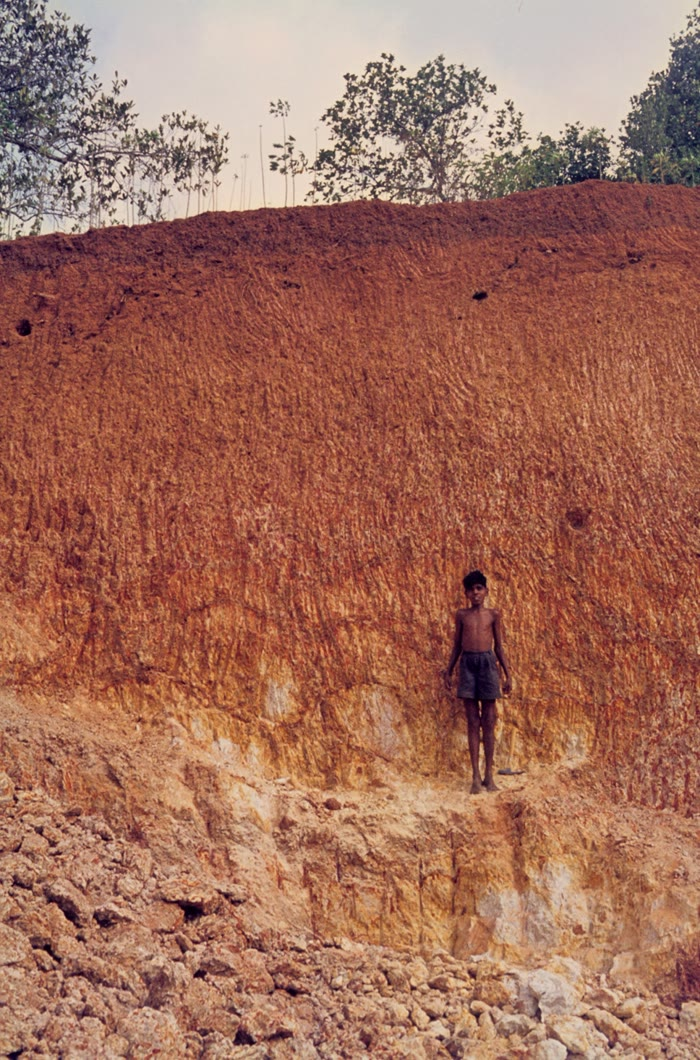
\includegraphics[height=8.5cm]{images/book2/g10-laterite-kerala.jpg}

{\small Um perfil de intemperismo sobre gnaisse granítico em Kerala, no sul
da Índia: embaixo, uma rocha decomposta e mosqueada; acima, uma \omterm{def:g10:soil-formation:laterite}{laterita}
marrom, fracamente endurecida, sob um solo fino. O menino dá a escala.
Fotografia: Werner Schellmann, 1969 (CC~BY-SA~2.5).}
\end{omfigure}

\begin{recall}
O intemperismo fragmenta as rochas onde elas estão; a erosão leva os
pedaços embora; a deposição os assenta em outro lugar (Livro 1, 5º ano). As
rochas são feitas de minerais, como o quartzo, os feldspatos e as micas de
um granito (Livro 1, 6º ano). Um solo é uma camada viva de grãos minerais,
húmus, água, ar e organismos; os decompositores transformam a matéria morta
em húmus; um solo é descrito pelas suas camadas, ou horizontes (os livros de
biologia). Numa oxidação, uma substância perde elétrons, muitas vezes ao se
combinar com o oxigênio (os livros de química).
\end{recall}

\section{Da rocha ao solo}

O intemperismo físico --- a cunha de gelo, o aquecimento e o resfriamento,
as raízes --- quebra a rocha em pedaços sem mudar os seus minerais. O
\omterm{def:g10:soil-formation:chemical-weathering}{intemperismo químico} muda os próprios minerais. Juntos, ao longo de tempos
longos, eles transformam o topo da rocha sólida num manto solto que se
espessa para baixo à medida que o intemperismo avança na rocha de baixo.

\begin{definition}[Rocha-mãe; saprolito]\label{def:g10:soil-formation:weathering-profile}
A \emph{rocha-mãe}\index{rocha-mae@rocha-mãe} de um solo é a rocha a partir
da qual a sua parte mineral se formou. O \emph{saprolito}\index{saprolito} é
a rocha decomposta no lugar pelo intemperismo: mole e terrosa, ela ainda
mostra os grãos e a estrutura da rocha-mãe. Um \emph{perfil de
intemperismo} é a coluna inteira, da rocha fresca, passando pelo saprolito,
até o solo no topo.
\end{definition}
% ledger: usgs:saprolite

O \omterm{def:g10:soil-formation:weathering-profile}{saprolito} pode ser espesso. Sob as colinas onduladas ao longo do lado
leste dos Montes Apalaches, no leste dos Estados Unidos, ele chega a cerca
de \qty{46}{m} (150 pés) em alguns lugares, embora a sua espessura varie
muito de um lugar para outro; o solo é só a parte de cima dele.
% ledger: usgs:saprolite

\begin{omfigure}
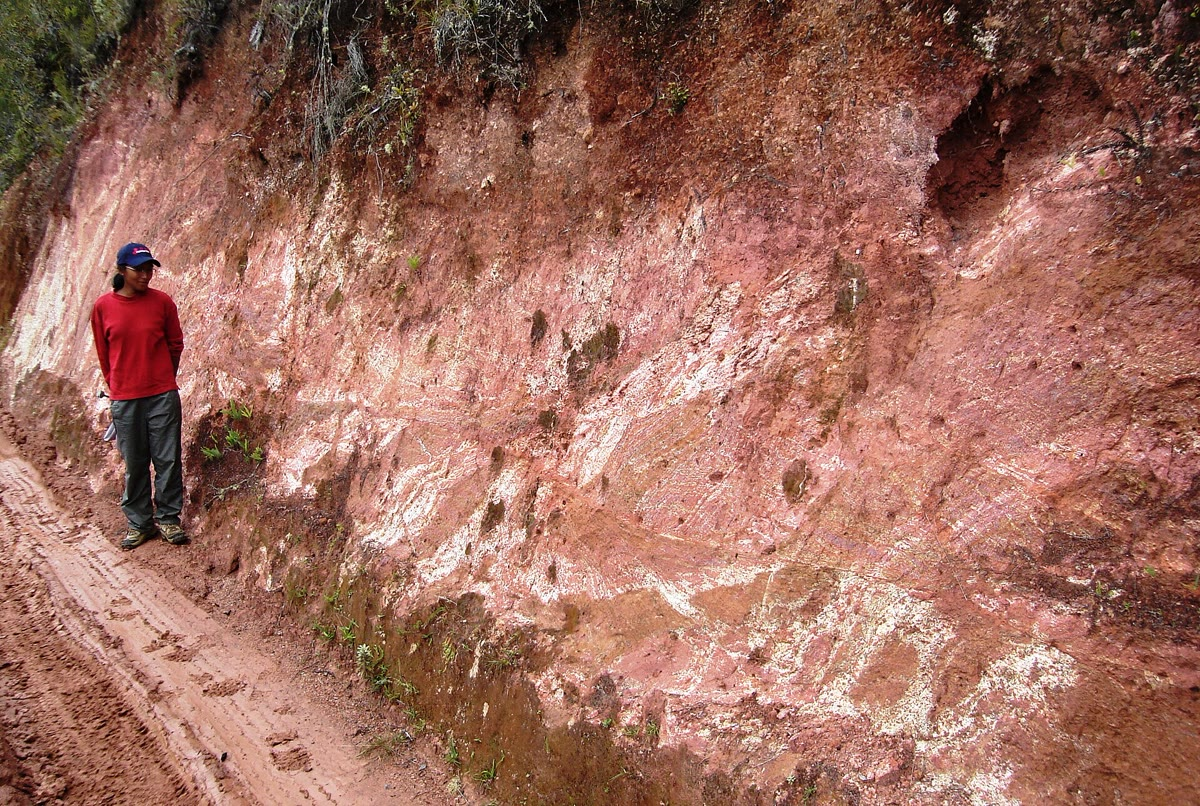
\includegraphics[width=0.8\linewidth]{images/book2/g10-saprolite-madagascar.jpg}

{\small \omterm{def:g10:soil-formation:weathering-profile}{Saprolito} num corte de estrada no centro de Madagascar: o antigo
gnaisse, decomposto no lugar, ainda mostra as suas bandas como listras de
argila branca na terra vermelha. Fotografia: Diorit (CC~BY-SA~3.0).}
\end{omfigure}

\begin{omfigure}
\begin{tikzpicture}[font=\footnotesize]
  % humid tropical column
  \begin{scope}
    \fill[omThm!45!brown!60] (0,5.4) rectangle (1.8,6.0);
    \fill[omThm!70!orange!70] (0,4.2) rectangle (1.8,5.4);
    \fill[omThm!25!orange!35] (0,1.2) rectangle (1.8,4.2);
    \foreach \y in {1.5,2.1,2.7,3.3,3.9} \draw[white!80!black, thick] (0.1,\y) -- (1.7,\y+0.15);
    \fill[black!30] (0,0) rectangle (1.8,1.2);
    \foreach \x/\y in {0.3/0.3,0.9/0.7,1.4/0.2,0.5/0.9,1.2/1.0} \draw[black!55] (\x,\y) -- ++(0.2,0.08);
    \draw[black!60] (0,0) rectangle (1.8,6.0);
    \node[anchor=north, align=center] at (0.9,-0.1) {trópicos úmidos};
  \end{scope}
  % temperate column
  \begin{scope}[xshift=3.2cm]
    \fill[omThm!45!brown!60] (0,2.2) rectangle (1.8,2.6);
    \fill[omThm!25!orange!35] (0,1.2) rectangle (1.8,2.2);
    \foreach \y in {1.5,1.9} \draw[white!80!black, thick] (0.1,\y) -- (1.7,\y+0.15);
    \fill[black!30] (0,0) rectangle (1.8,1.2);
    \foreach \x/\y in {0.3/0.3,0.9/0.7,1.4/0.2,0.5/0.9,1.2/1.0} \draw[black!55] (\x,\y) -- ++(0.2,0.08);
    \draw[black!60] (0,0) rectangle (1.8,2.6);
    \node[anchor=north, align=center] at (0.9,-0.1) {clima\\temperado};
  \end{scope}
  % labels
  \draw[black!50] (5.3,5.7) -- (2.0,5.7); \node[anchor=west] at (5.4,5.7) {solo};
  \draw[black!50] (5.3,4.8) -- (2.0,4.8); \node[anchor=west, align=left] at (5.4,4.8) {laterita: vermelha, rica em óxidos\\de ferro e de alumínio};
  \draw[black!50] (5.3,3.4) -- (2.0,3.4); \node[anchor=west, align=left] at (5.4,3.4) {saprolito: rocha decomposta\\no lugar, estrutura conservada};
  \draw[black!50] (5.3,0.6) -- (5.0,0.6); \node[anchor=west] at (5.4,0.6) {rocha-mãe fresca};
\end{tikzpicture}

{\small Dois perfis de intemperismo sobre a mesma rocha (esquema, fora de
escala): sob um clima quente e úmido, o perfil é muito mais espesso e o seu
topo é uma \omterm{def:g10:soil-formation:laterite}{laterita}; sob um clima temperado, um \omterm{def:g10:soil-formation:weathering-profile}{saprolito} mais fino sustenta
o solo.}
\end{omfigure}

\section{O intemperismo químico}

\begin{definition}[Intemperismo químico]\label{def:g10:soil-formation:chemical-weathering}
O \emph{intemperismo químico}\index{intemperismo quimico@intemperismo químico}
é a transformação dos minerais de uma rocha por reações com a água e com os
gases que ela leva, o gás carbônico e o oxigênio: alguns minerais se
dissolvem, outros são transformados em minerais novos, estáveis na
superfície da Terra.
\end{definition}

A água da chuva dissolve um pouco de gás carbônico do ar, e muito mais ao se
infiltrar pelo solo, onde as raízes e os decompositores o expiram. Parte do
gás dissolvido forma ácido carbônico, que libera íons hidrogênio:
\begin{center}
\ce{CO2 + H2O -> H+ + HCO3-}
\end{center}
Esses íons hidrogênio atacam os minerais.

\begin{definition}[Hidrólise]\label{def:g10:soil-formation:hydrolysis}
A \emph{hidrólise}\index{hidrolise@hidrólise} é o \omterm{def:g10:soil-formation:chemical-weathering}{intemperismo químico} de um
mineral silicático pela água e pelos seus íons hidrogênio: os íons hidrogênio
tomam o lugar dos íons metálicos do mineral, que passam para a solução, e o
restante do mineral é reconstruído num \omterm{def:g10:soil-formation:clay}{argilomineral}.
\end{definition}

\begin{proposition}[Hidrólise de um feldspato]\label{prop:g10:soil-formation:hydrolysis}
O feldspato potássico ortoclásio, \ce{KAlSi3O8}, é transformado por \omterm{def:g10:soil-formation:hydrolysis}{hidrólise}
no \omterm{def:g10:soil-formation:clay}{argilomineral} caulinita, \ce{Al2Si2O5(OH)4}; os íons potássio e a sílica
dissolvida, \ce{H4SiO4}, são levados pela água:
\begin{center}
\ce{2 KAlSi3O8 + 2 H+ + 9 H2O -> Al2Si2O5(OH)4 + 2 K+ + 4 H4SiO4}
\end{center}
\end{proposition}
% ledger: webmineral:formulas

\begin{proof}[Verificação]
Conte cada elemento dos dois lados. Potássio: 2 e 2. Alumínio: 2 e 2.
Silício: 6 e $2 + 4 = 6$. Oxigênio: $16 + 9 = 25$ e $9 + 16 = 25$.
Hidrogênio: $2 + 18 = 20$ e $4 + 16 = 20$. Carga: $+2$ e $+2$.
\end{proof}

\begin{proposition}[Dissolução da calcita]\label{prop:g10:soil-formation:calcite}
A calcita, \ce{CaCO3}, o mineral do calcário, se dissolve completamente na
água que leva gás carbônico; nada sólido sobra:
\begin{center}
\ce{CaCO3 + CO2 + H2O -> Ca^2+ + 2 HCO3-}
\end{center}
\end{proposition}
% ledger: webmineral:formulas

O ferro é atacado de uma terceira maneira. Nos minerais escuros de uma rocha,
como a mica preta de um granito, o ferro está na forma reduzida \ce{Fe^2+}.
O oxigênio levado pela água o oxida, e o ferro(III) fica para trás como
óxidos insolúveis: a goethita, amarelo-amarronzada, \ce{FeO(OH)}, e a
hematita, vermelha, \ce{Fe2O3}. Para a goethita:
\begin{center}
\ce{4 Fe^2+ + O2 + 6 H2O -> 4 FeO(OH) + 8 H+}
\end{center}
Esses óxidos colorem as rochas intemperizadas e os solos de amarelo, marrom
e vermelho.
% ledger: webmineral:formulas

Nem todos os minerais se alteram no mesmo ritmo. Num granito em
intemperismo, a mica preta enferruja e os feldspatos se transformam em
argila, mas os grãos de quartzo, quase insolúveis, saem intactos: eles
acabam como areia.

\begin{example}[O intemperismo de um granito]\label{ex:g10:soil-formation:granite}
% ledger: webmineral:formulas (masses computed in figdata/grade-10/soil_rates.py)
Um quilograma de ortoclásio contém $1000/278.33 \approx \qty{3.59}{mol}$ de
\ce{KAlSi3O8}. Pela equação, dois mols de ortoclásio dão um mol de
caulinita: $3.59/2 \approx \qty{1.80}{mol}$, isto é, $1.80 \times 258.16
\approx \qty{464}{g}$ de argila. O potássio, $14.05~\%$ da massa do
ortoclásio, \qty{140.5}{g}, e $2 \times 3.59 = \qty{7.19}{mol}$ de sílica
saem em solução. De um granito de quartzo, feldspatos e micas, o
intemperismo deixa areia (o quartzo), argila (dos feldspatos e das micas) e
óxidos de ferro, e manda potássio, sódio, cálcio e sílica para os rios.
\end{example}

\section{As argilas e o húmus}

\begin{definition}[Argilomineral]\label{def:g10:soil-formation:clay}
Um \emph{argilomineral}\index{argilomineral} é um silicato formado de folhas
finas de átomos empilhadas umas sobre as outras, produzido pelo
intemperismo, que ocorre em lâminas muito menores que os grãos de areia. A
caulinita é um deles.
\end{definition}
% ledger: webmineral:formulas

As superfícies das lâminas de argila levam cargas elétricas negativas. Elas
retêm íons positivos --- potássio \ce{K+}, cálcio \ce{Ca^2+}, magnésio
\ce{Mg^2+}, amônio \ce{NH4+} --- que de outro modo seriam lavados pela
chuva. O húmus faz o mesmo. Ligados, a argila e o húmus formam o
\emph{complexo argilo-húmico}, a reserva de nutrientes minerais do solo: uma
raiz libera íons hidrogênio e recebe em troca o potássio ou o cálcio retido
nas lâminas.

\begin{omfigure}
\begin{tikzpicture}[font=\footnotesize, >={Stealth[length=2mm]}]
  \foreach \y in {0,0.7,1.4} {
    \fill[omExo!35, draw=black!60] (0,\y) rectangle (7.2,\y+0.3);
    \foreach \x in {0.3,0.9,...,7.0} \node[font=\tiny, black!70] at (\x,\y+0.15) {$-$};
  }
  \foreach \x/\ion in {0.7/K^+, 1.9/Ca^{2+}, 3.1/K^+, 4.3/Mg^{2+}, 5.5/NH_4^+, 6.7/K^+} {
    \fill[omThm!20, draw=omThm!80!black] (\x,2.1) circle (0.4);
    \node[font=\scriptsize] at (\x,2.1) {$\mathrm{\ion}$};
  }
  \foreach \x in {1.3, 3.7, 6.1} \fill[omThm!20, draw=omThm!80!black] (\x,0.5) circle (0.17);
  \foreach \x in {2.5, 4.9} \fill[omThm!20, draw=omThm!80!black] (\x,1.2) circle (0.17);
  \node[anchor=north] at (3.6,-0.1) {folhas de argila, de carga negativa, com íons positivos entre elas};
  \node[anchor=south] at (3.1,2.5) {íons positivos retidos nas superfícies};
  % root and exchange
  \draw[line width=2.2pt, brown!60!black] (9.6,3.4) .. controls (9.3,2.6) and (8.9,2.2) .. (8.1,2.0);
  \node[anchor=east] at (9.25,3.3) {raiz};
  \draw[->, omDef!80!black, thick] (8.0,2.2) .. controls (7.6,2.6) and (7.2,2.6) .. (6.95,2.3);
  \node[anchor=south, omDef!80!black] at (7.5,2.55) {\ce{H+} cedido};
  \draw[->, omThm!80!black, thick] (6.95,1.8) .. controls (7.3,1.5) and (7.7,1.6) .. (8.0,1.85);
  \node[anchor=north, omThm!80!black] at (7.8,1.55) {\ce{K+} tomado};
\end{tikzpicture}

{\small O complexo argilo-húmico (esquema): folhas de argila de carga
negativa retêm íons positivos nas suas superfícies e entre elas; uma raiz
troca íons hidrogênio por esses nutrientes.}
\end{omfigure}

\section{Os solos e o clima}

O \omterm{def:g10:soil-formation:chemical-weathering}{intemperismo químico} precisa de água e, como a maioria das reações, anda
mais depressa quando faz calor. Onde o clima é ao mesmo tempo quente e
úmido, a rocha se decompõe mais fundo e mais completamente: os feldspatos se
transformam inteiramente em argila, até boa parte da sílica é levada embora,
e o que sobra é rico nos elementos menos solúveis, o ferro e o alumínio.

\begin{definition}[Laterita]\label{def:g10:soil-formation:laterite}
Uma \emph{laterita}\index{laterita} é um material profundamente
intemperizado dos climas quentes e úmidos, vermelho ou marrom, feito
principalmente de óxidos de ferro e de alumínio e de caulinita, do qual
quase tudo o que é solúvel foi removido.
\end{definition}

Sob climas frios, congelados durante boa parte do ano, e sob climas secos,
onde a água é escassa, o \omterm{def:g10:soil-formation:chemical-weathering}{intemperismo químico} é lento: os solos são finos e
a rocha fica logo abaixo. Entre os polos e o equador, a profundidade do
intemperismo é máxima sob as florestas tropicais úmidas e mínima nos
desertos e nas regiões polares.

\begin{omfigure}
\begin{tikzpicture}[font=\footnotesize]
  \fill[black!25] (0,-0.2) -- (0,-0.5) .. controls (1.5,-0.6) and (2.5,-1.4) .. (3.4,-1.2)
     .. controls (4.2,-1.0) and (4.6,-0.55) .. (5.2,-0.5) .. controls (6.0,-0.5) and (6.6,-1.6) .. (7.6,-3.0)
     .. controls (8.2,-3.6) and (9.0,-3.6) .. (10,-3.4) -- (10,-3.8) -- (0,-3.8) -- cycle;
  \fill[omThm!25!orange!35] (0,0) -- (10,0) -- (10,-3.4) .. controls (9.0,-3.6) and (8.2,-3.6) .. (7.6,-3.0)
     .. controls (6.6,-1.6) and (6.0,-0.5) .. (5.2,-0.5) .. controls (4.6,-0.55) and (4.2,-1.0) .. (3.4,-1.2)
     .. controls (2.5,-1.4) and (1.5,-0.6) .. (0,-0.5) -- cycle;
  \draw[black!60] (0,0) -- (10,0);
  \node[anchor=south] at (0.6,0.05) {polar};
  \node[anchor=south] at (3.2,0.05) {temperado};
  \node[anchor=south] at (5.3,0.05) {deserto};
  \node[anchor=south] at (6.8,0.05) {savana};
  \node[anchor=south] at (9.0,0.05) {floresta tropical};
  \node[anchor=north] at (0.4,-3.85) {polo};
  \node[anchor=north] at (9.6,-3.85) {equador};
  \node[black!70] at (2.0,-2.6) {rocha fresca};
  \node[black!80] at (8.35,-1.0) {rocha intemperizada e solo};
\end{tikzpicture}

{\small A profundidade do intemperismo de um polo ao equador (esquema,
profundidades fora de escala): pequena sob os climas polares e desérticos,
moderada sob os climas temperados, máxima sob as florestas tropicais
úmidas.}
\end{omfigure}

\section{Lento para se formar, rápido para se perder}

Com que rapidez o solo se forma? A produção de solo, a taxa com que o
intemperismo transforma a rocha em solo na base do perfil, foi medida em
muitos lugares do mundo, assim como a taxa com que o solo é erodido na
superfície. Uma compilação dessas medições dá as taxas típicas (medianas)
abaixo, cada uma expressa como uma espessura de solo por ano.
% ledger: montgomery:rates

\begin{omfigure}
\begin{tikzpicture}
\begin{axis}[omrecord, width=0.82\linewidth, height=5.6cm, ymode=log, log origin=infty, ymin=0.005,
  ymax=5, ybar, bar width=16pt, xtick={0,1,2,3,4}, xmin=-0.6, xmax=4.6,
  xticklabels={{produção\\de solo}, {erosão sob\\vegetação nativa}, {erosão\\geológica}, {agricultura\\de conservação}, {aração\\convencional}},
  xticklabel style={align=center, font=\scriptsize},
  ylabel={taxa (\unit{mm} por ano)}, tick label style={font=\small}, label style={font=\small},
  nodes near coords, nodes near coords style={font=\scriptsize}, point meta=explicit symbolic]
\addplot[fill=omDef!45, draw=omDef!80!black] table[x=idx, y=rate_mm_yr, meta=rate_mm_yr] {figdata/out/grade-10-soil_rates-rates.dat};
\end{axis}
\end{tikzpicture}

{\small Taxas medianas de produção de solo e de erosão de uma compilação
mundial de medições, em milímetros de solo por ano (escala logarítmica: cada
degrau vale dez vezes o de baixo). Dados: Montgomery
(2007), revista \emph{Proceedings of the National Academy of Sciences}.}
\end{omfigure}
% ledger: montgomery:rates

Sob a vegetação natural, o solo é erodido mais ou menos tão depressa quanto
se forma, cerca de \qty{0.02}{mm} por ano: um centímetro em uns seis séculos.
Sob a aração convencional, que deixa o chão nu entre as culturas, a taxa
mediana de erosão é de \qty{1.5}{mm} por ano, noventa vezes a taxa de
produção de solo. Sob a agricultura de conservação, que perturba menos o
solo e o mantém coberto, a mediana cai para \qty{0.08}{mm} por ano, muito
mais perto da taxa de produção.
% ledger: montgomery:rates (ratios computed in figdata/grade-10/soil_rates.py)

\begin{method}[Comparar uma taxa de formação com uma taxa de erosão]\label{met:g10:soil-formation:rates}
\begin{enumerate}
  \item Exprima as duas taxas na mesma unidade (milímetros por ano).
  \item A perda líquida é a taxa de erosão $E$ menos a taxa de produção $P$.
  \item Um solo de espessura $S$ é perdido em $T = S/(E - P)$ anos; se
        $E \le P$, o solo não está sendo perdido.
  \item Formar uma espessura $S$ a partir do zero leva $S/P$ anos.
\end{enumerate}
\end{method}
% ledger: montgomery:lifetime

Com essas taxas, um metro de solo leva cerca de $1000/0.017 \approx 59\,000$
anos para se formar, e sob a aração convencional ele pode ser perdido em
cerca de $1000/(1.537 - 0.017) \approx 660$ anos. Nas escalas de tempo
humanas, o solo é um recurso que não se renova.
% ledger: montgomery:rates, montgomery:lifetime

\begin{omfigure}
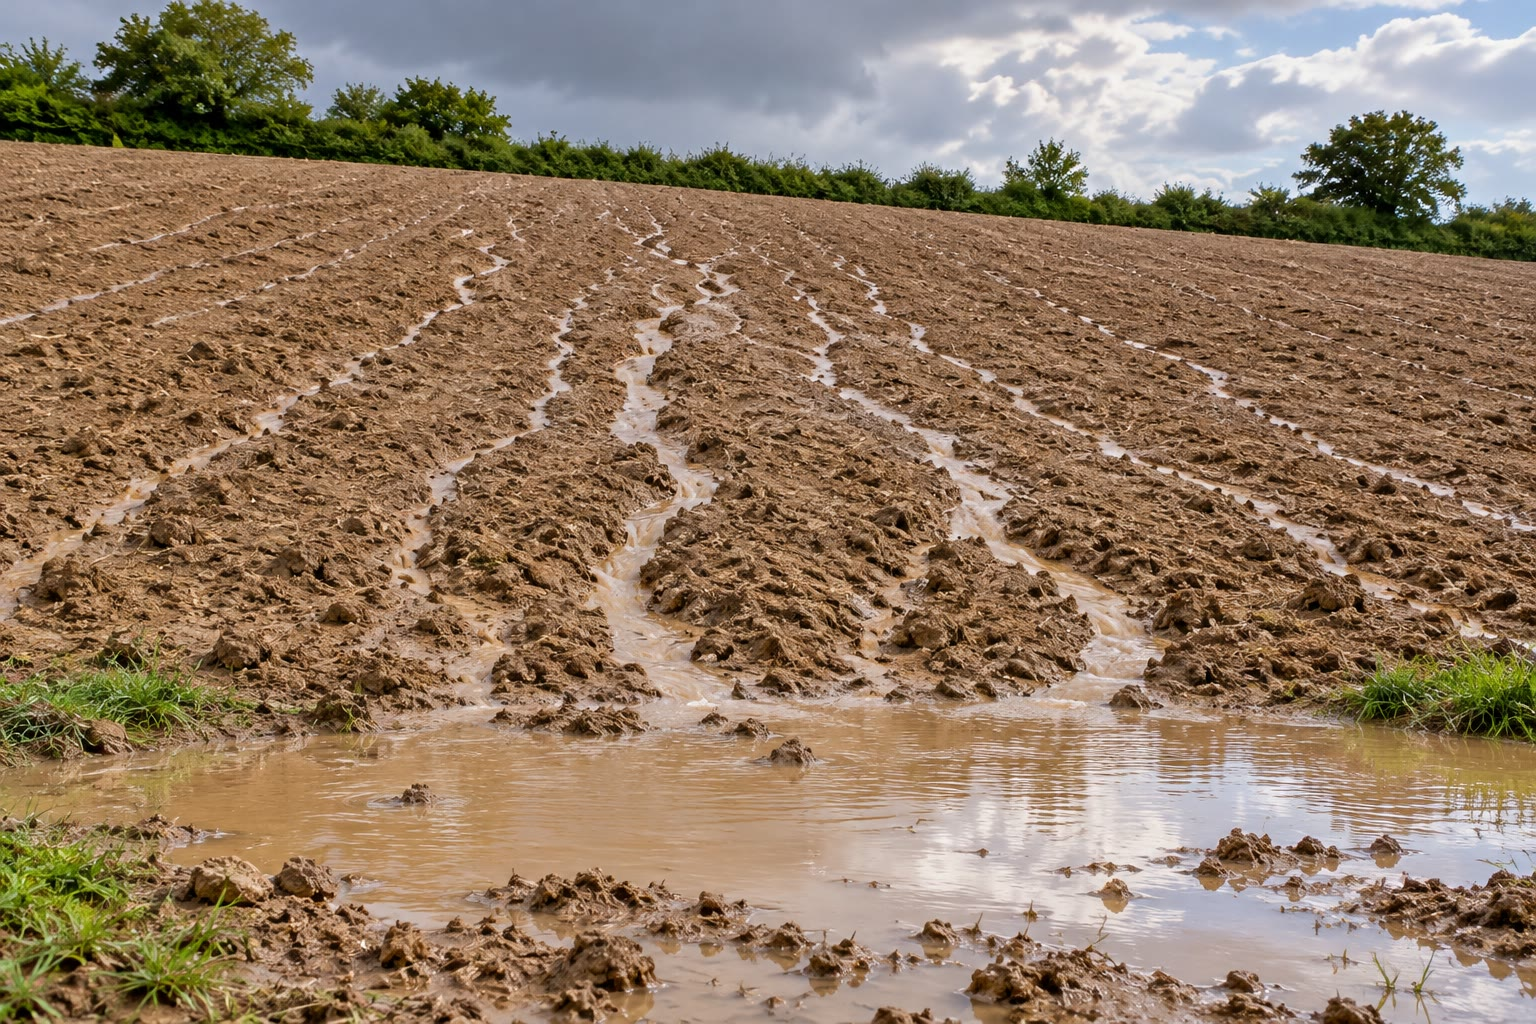
\includegraphics[width=0.72\linewidth]{images/book2/ai/g10-ploughed-rills.jpg}

{\small Um campo arado depois de uma chuva forte: o escoamento abriu
pequenos canais, ou sulcos, encosta abaixo e levou o solo para uma poça
lamacenta no seu pé.}
\end{omfigure}

\section{Exercícios}

\begin{exercise}[$\star$]\label{exo:g10:soil-formation:1}
Defina o \omterm{def:g10:soil-formation:chemical-weathering}{intemperismo químico} e a \omterm{def:g10:soil-formation:hydrolysis}{hidrólise}.
\end{exercise}

\begin{exercise}[$\star$]\label{exo:g10:soil-formation:2}
O que é o \omterm{def:g10:soil-formation:weathering-profile}{saprolito}? Como distinguir o \omterm{def:g10:soil-formation:weathering-profile}{saprolito} de um solo formado em areia
trazida por um rio?
\end{exercise}

\begin{exercise}[$\star$]\label{exo:g10:soil-formation:3}
Dê o nome dos produtos do intemperismo de um granito: em que se transforma
cada um dos seus três minerais principais?
\end{exercise}

\begin{exercise}[$\star$]\label{exo:g10:soil-formation:4}
Por que as rochas intemperizadas e os solos tropicais são tão frequentemente
vermelhos, amarelos ou marrons?
\end{exercise}

\begin{exercise}[$\star$]\label{exo:g10:soil-formation:5}
Usando o gráfico de barras, dê a taxa mediana de produção de solo e a taxa
mediana de erosão sob a aração convencional. Quantas vezes maior é a
segunda?
\end{exercise}

\begin{exercise}[$\star\star$]\label{exo:g10:soil-formation:6}
Verifique que a equação da dissolução da calcita está balanceada, para cada
elemento e para a carga.
\end{exercise}

\begin{exercise}[$\star\star$]\label{exo:g10:soil-formation:7}
O calcário se dissolve completamente, o granito deixa areia e argila.
Explique a diferença usando as duas reações do capítulo.
\end{exercise}

\begin{exercise}[$\star\star$]\label{exo:g10:soil-formation:8}
Explique como o complexo argilo-húmico retém o potássio num solo que a chuva
atravessa, e como uma raiz o obtém.
\end{exercise}

\begin{exercise}[$\star\star$]\label{exo:g10:soil-formation:9}
Dê duas razões pelas quais as \omterm{def:g10:soil-formation:laterite}{lateritas} se formam sob climas quentes e
úmidos, e não sob climas frios ou secos.
\end{exercise}

\begin{exercise}[$\star\star$]\label{exo:g10:soil-formation:10}
A taxa mediana de produção de solo é de \qty{0.017}{mm} por ano. Quanto
tempo leva para formar \qty{1}{cm}, \qty{30}{cm} e \qty{1}{m} de solo?
\end{exercise}

\begin{exercise}[$\star\star$]\label{exo:g10:soil-formation:11}
As taxas de erosão são muitas vezes dadas como uma massa de solo por hectare
por ano. Com uma densidade do solo de \qty{1200}{kg/m^3}, que massa uma
perda de \qty{1.5}{mm} por ano representa num hectare (\qty{10000}{m^2})?
\end{exercise}

\begin{exercise}[$\star\star\star$]\label{exo:g10:soil-formation:12}
Um \omterm{def:g10:soil-formation:weathering-profile}{saprolito} de \qty{46}{m} de espessura se formou sob as colinas de uma
região temperada. Se o intemperismo avançasse na rocha a \qty{0.017}{mm} por
ano, quanto tempo isso teria levado? O que a resposta sugere sobre a idade
de uma paisagem assim?
\end{exercise}

\begin{exercise}[$\star\star\star$]\label{exo:g10:soil-formation:13}
Escreva a equação da oxidação do \ce{Fe^2+} em goethita dada no capítulo e
verifique-a. Depois escreva e balanceie a oxidação do \ce{Fe^2+} em
hematita, \ce{Fe2O3}, pelo oxigênio e pela água, liberando \ce{H+}.
\end{exercise}

\begin{exercise}[$\star\star\star$]\label{exo:g10:soil-formation:14}
Sob a agricultura de conservação, a taxa mediana de erosão é de
\qty{0.082}{mm} por ano. Com a produção de solo a \qty{0.017}{mm} por ano,
quanto tempo leva para perder \qty{30}{cm} de solo? Compare com a aração
convencional.
\end{exercise}

\begin{exercise}[$\star\star\star$]\label{exo:g10:soil-formation:15}
Um granito contém \qty{30}{\percent} de ortoclásio em massa. Que massa de
caulinita se forma quando todo o ortoclásio de uma tonelada desse granito
foi intemperizado, e que massa de potássio é liberada?
\end{exercise}

\section{Problema: o tempo de vida de um solo}

\begin{problem}[{Problema de fim de semana --- da rocha ao campo e de volta ao rio}]
\label{pb:g10:soil-formation:1}
% ledger: montgomery:rates, montgomery:lifetime, webmineral:formulas (values computed in figdata/grade-10/soil_rates.py)

\begin{center}
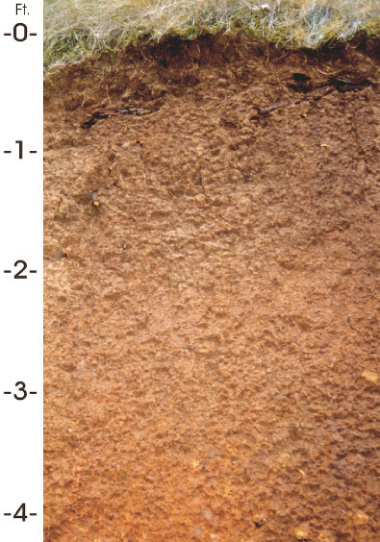
\includegraphics[height=6cm]{images/book2/g10-nrcs-jory-soil.jpg}

{\small Um perfil de solo, com uma escala em pés à esquerda (\num{1}~pé =
\qty{0.3048}{m}). Fotografia: USDA Natural Resources Conservation Service
(domínio público).}
\end{center}

\medskip
\noindent\textbf{Parte I --- Um perfil.}
\begin{enumerate}
  \item A escala chega a 4 pés perto da base da imagem. A que profundidade
        isso corresponde, em metros?
  \item A camada escura do topo chega a cerca de meio pé. Qual é a sua
        espessura, em centímetros?
  \item O que dá a essa camada do topo a sua cor escura?
  \item Abaixo, o solo é marrom-avermelhado. Que minerais lhe dão essa cor, e
        como eles se formaram?
  \item A \omterm{def:g10:soil-formation:weathering-profile}{rocha-mãe} é visível na fotografia? O que você esperaria encontrar
        abaixo da base da imagem?
\end{enumerate}

\medskip
\noindent\textbf{Parte II --- A química de um granito em intemperismo.}
\begin{enumerate}[resume]
  \item Escreva a equação da \omterm{def:g10:soil-formation:hydrolysis}{hidrólise} do ortoclásio.
  \item Quantos mols de ortoclásio há em \qty{1}{kg}
        (\qty{278.33}{g/mol})?
  \item Que massa de caulinita (\qty{258.16}{g/mol}) eles dão?
  \item O que sai na água, e para onde vai?
  \item O que acontece com o quartzo do granito?
\end{enumerate}

\medskip
\noindent\textbf{Parte III --- Formação contra erosão.}
\begin{enumerate}[resume]
  \item O solo se forma a \qty{0.017}{mm} por ano. Quanto tempo leva para
        formar o perfil da Parte I?
  \item Sob a aração convencional, o solo é erodido a \qty{1.537}{mm} por
        ano. Qual é a perda líquida a cada ano?
  \item Quanto tempo duraria o perfil da Parte I?
  \item Compare os dois tempos das questões 11 e 13.
  \item Sob a vegetação natural, a erosão é de \qty{0.013}{mm} por ano. O
        solo está sendo perdido?
\end{enumerate}

\medskip
\noindent\textbf{Parte IV --- O tempo de vida do solo.}
\begin{enumerate}[resume]
  \item Escreva o tempo $T$ para perder uma espessura $S$ de solo em função
        de $S$, da taxa de erosão $E$ e da taxa de produção $P$.
  \item Calcule $T$ para $S = \qty{30}{cm}$ sob a aração convencional.
  \item Calcule $T$ para $S = \qty{30}{cm}$ sob a agricultura de conservação
        (\qty{0.082}{mm} por ano).
  \item Por que se pode dizer que um solo é um recurso que não se renova nas
        escalas de tempo humanas?
  \item Quanto tempo leva para perder um metro de solo sob a aração
        convencional?
\end{enumerate}
\end{problem}
